% Standalone source of Fig. 1. Compiled to fig_architecture.pdf by build_paper.py.
\documentclass[tikz,border=1pt]{standalone}
\usepackage[T1]{fontenc}
\usepackage{newtxtext}
\usetikzlibrary{positioning,arrows.meta,fit,backgrounds}
\begin{document}
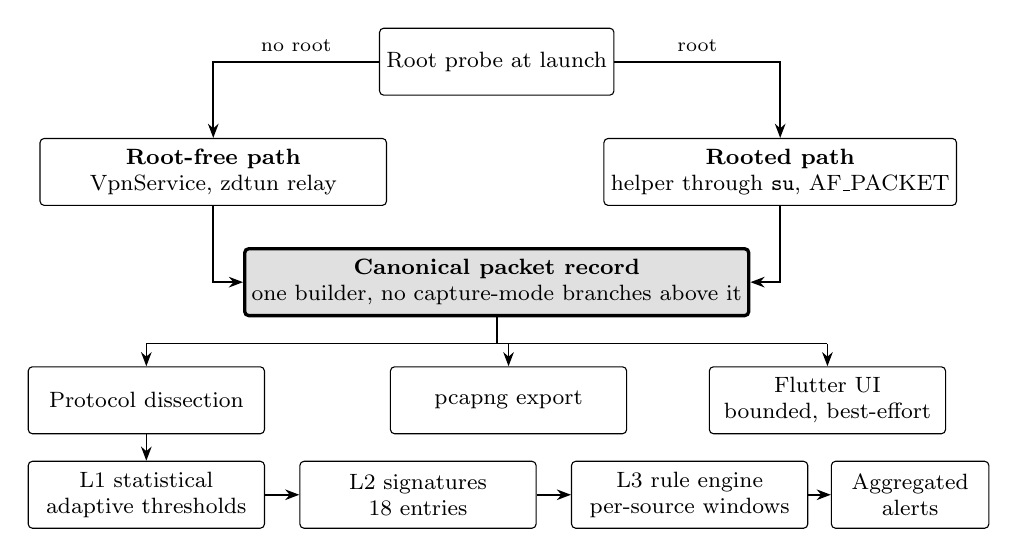
\begin{tikzpicture}[
  font=\footnotesize,
  box/.style={draw, rounded corners=1.5pt, align=center, minimum height=8.5mm, inner sep=2.5pt},
  arr/.style={-{Stealth[length=1.8mm]}, semithick},
  note/.style={font=\scriptsize, align=center}
]
% capture tier
\node[box] (probe) at (6,2.45) {Root probe at launch};
\node[box, minimum width=44mm] (vpn) at (2.4,1.05) {\textbf{Root-free path}\\VpnService, zdtun relay};
\node[box, minimum width=44mm] (root) at (9.6,1.05) {\textbf{Rooted path}\\helper through \texttt{su}, AF\_PACKET};
\draw[arr] (probe.west) -| node[note, above, pos=0.25] {no root} (vpn.north);
\draw[arr] (probe.east) -| node[note, above, pos=0.25] {root} (root.north);

% boundary
\node[box, very thick, fill=black!12, minimum width=64mm] (record) at (6,-0.35) {\textbf{Canonical packet record}\\one builder, no capture-mode branches above it};
\draw[arr] (vpn.south) |- (record.west);
\draw[arr] (root.south) |- (record.east);

% analysis tier
\node[box, minimum width=30mm] (dpi) at (1.55,-1.85) {Protocol dissection};
\node[box, minimum width=30mm] (l1) at (1.55,-3.05) {L1 statistical\\adaptive thresholds};
\node[box, minimum width=30mm] (l2) at (5.0,-3.05) {L2 signatures\\18 entries};
\node[box, minimum width=30mm] (l3) at (8.45,-3.05) {L3 rule engine\\per-source windows};
\node[box, minimum width=20mm] (alerts) at (11.25,-3.05) {Aggregated\\alerts};
\node[box, minimum width=30mm] (export) at (6.15,-1.85) {pcapng export};
\node[box, minimum width=30mm] (ui) at (10.2,-1.85) {Flutter UI\\bounded, best-effort};

\draw[semithick] (record.south) -- (6,-1.13);
\draw[semithick] (dpi.north |- 0,-1.13) -- (ui.north |- 0,-1.13);
\draw[arr] (dpi.north |- 0,-1.13) -- (dpi.north);
\draw[arr] (export.north |- 0,-1.13) -- (export.north);
\draw[arr] (ui.north |- 0,-1.13) -- (ui.north);
\draw[arr] (dpi.south) -- (l1.north);
\draw[arr] (l1.east) -- (l2.west);
\draw[arr] (l2.east) -- (l3.west);
\draw[arr] (l3.east) -- (alerts.west);
\end{tikzpicture}
\end{document}
